\chapter{Computational Methods}
\label{cha:methods}

As mentioned in the Introduction, the goal of this thesis is bringing computational cognitive models closer to being able to function in realistic environments under conditions of uncertainty, by proposing probabilistic models of spatial cognition which are implementable in brains. Probabilistic models have become successful and widespread in domains requiring the representation and manipulation of uncertainty, including artificial intelligence \citep{russell2009ai}, robotics \citep{thrun2005probabilistic}, and machine learning \citep{bishop2006pattern}. They have also been successfully employed in cognitive modelling  \citep{chater2010bayesian} and in neuroscience \citep{knill2004bayesian} - although there is little empirical evidence for particular neural implementations of probabilistic mechanisms as of yet \citep{griffiths2008bayesian, vilares2011bayesian, pouget2013probabilistic}. 

This section briefly reviews the computational methods employed in this thesis. Figure \ref{fig:methods} shows an overview over all employed methods, and the way they are utilized to support the mechanisms, algorithms, and cognitive models presented below. Figure \ref{fig:neurimpl} connects these computational mechanisms to their suggested implementation in brains (arguments and evidence for the neuroscientific plausibility of Bayesian localization are presented in Chapter \ref{cha:bayespc}). 

\begin{figure}[h]
	\centering
	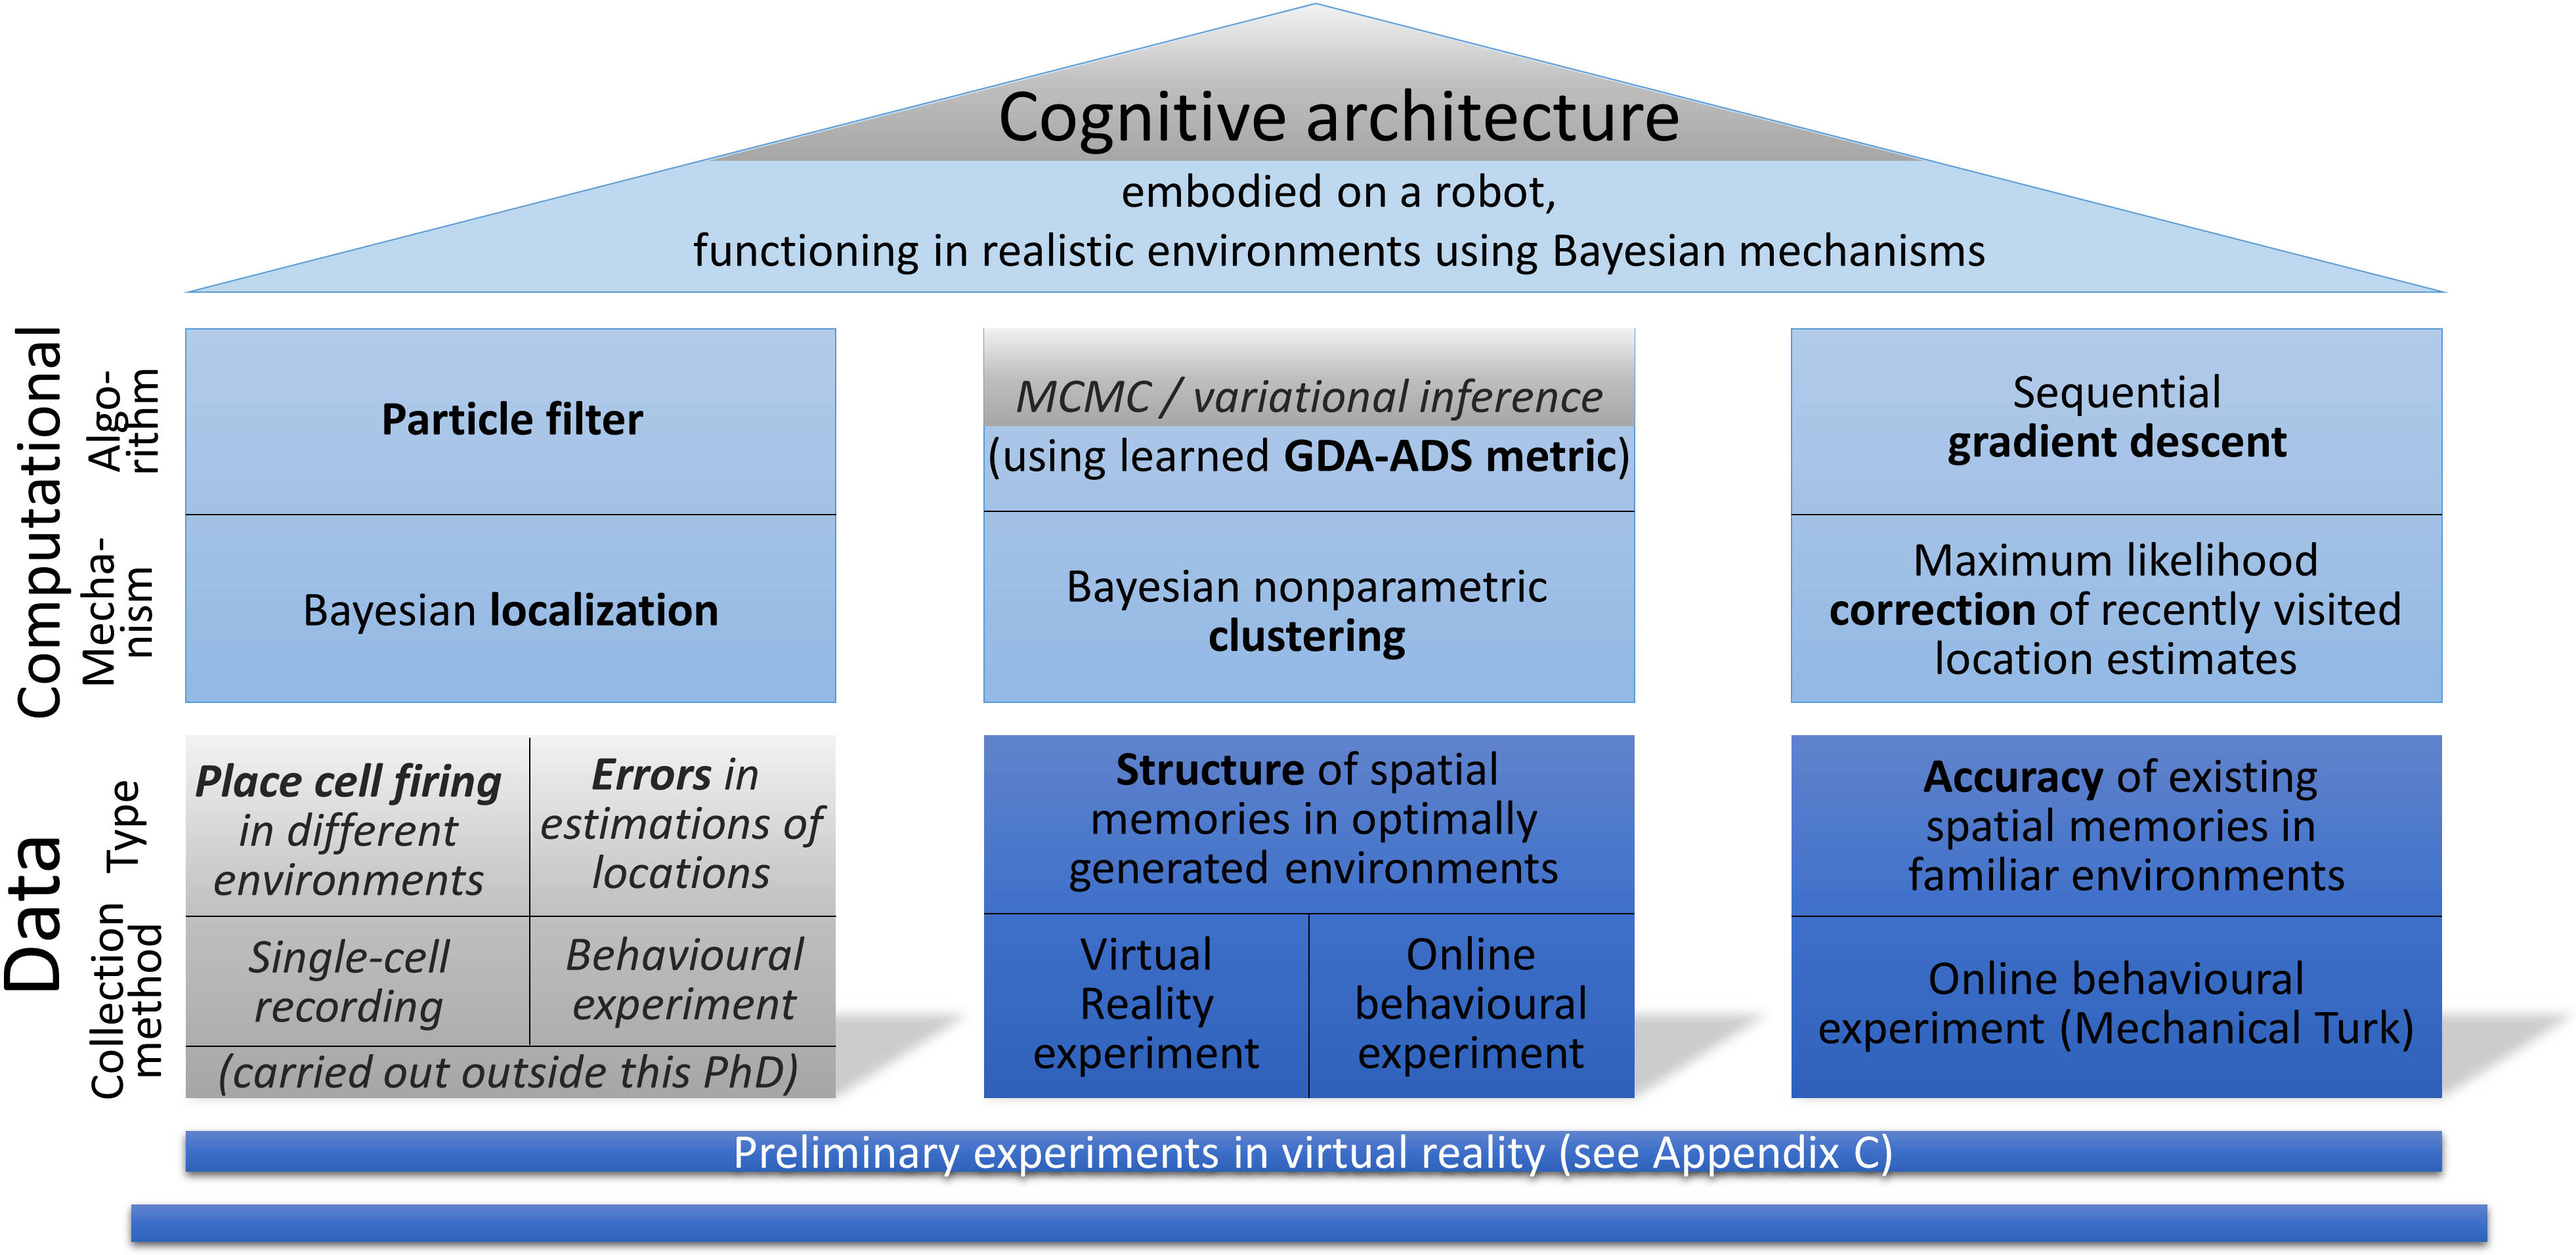
\includegraphics[width=\textwidth]{img/methodsfigure2}
	\caption[Overview of how the methods in this thesis help support real-world capable models of cognition]{\textbf{Overview of how the methods in this thesis help support real-world capable models of cognition,} roughly divided into empirical methods (bottom half) and computational methods (top half). Gray boxes contain data/code used to substantiate or implement some models, but not gathered/implemented by us.} 
	\label{fig:methods}
\end{figure}

To be able to plan novel routes in pursuit of its goals, an agent (whether biological or artificial), at a minimum, needs to be able to localize itself, its goal, and possible obstacles; and needs to do so in the face of a noisy and inaccurate sensory apparatus. From a probabilistic perspective, this localization problem can be described as a Bayesian network (see Figure \ref{fig:neurimpl}B). In order to avoid having to perform calculations over every location ever visited, and every landmark ever observed, as done in many robotics solutions \citep{durrant2006simultaneous,bailey2006simultaneous}, we split it into sub-problems. 

Specifically, an approximate solution of this problem can be split into Bayesian cue integration for integrating noisy observations into a location estimate (Section \ref{sec:bayescue}), Bayesian localization for maintaining this location estimate through time (Section \ref{sec:bayesloc}), and maximum likelihood-based correction for fixing the most recent location estimates when revisiting a location (Section \ref{sec:bayescorr}). We suggest a rejection sampling-based algorithm for the former two, implementable through coincidence detection in hippocampal place cells (Chapter \ref{cha:bayespc}), and a gradient descent-based solution for the latter, implementable by reverse replay in the hippocampus (Chapter \ref{cha:lida}). We will present empirical evidence for these claims in those chapters, both from single-neuron recordings in live animals (collected outside this PhD) and from behavioural experiments performed online with participants recruited from Amazon's Mechanical Turk\footnote{https://www.mturk.com}.

These mechanisms help inferring spatial locations in the environment from noisy observations, in a neurally and psychologically plausible fashion, as we will argue below. However, in a system operating under limited time and resources, these locations also need to be stored efficiently, such that they can be rapidly accessed. Hierarchical representations facilitate such desirable properties, and have been argued to be prevalent in human cognition \citep{cohen2000hierarchical, gobet2001chunking}. There is strong evidence

\nocite{deshmukh2013}

\begin{figure}[h]
	\centering
	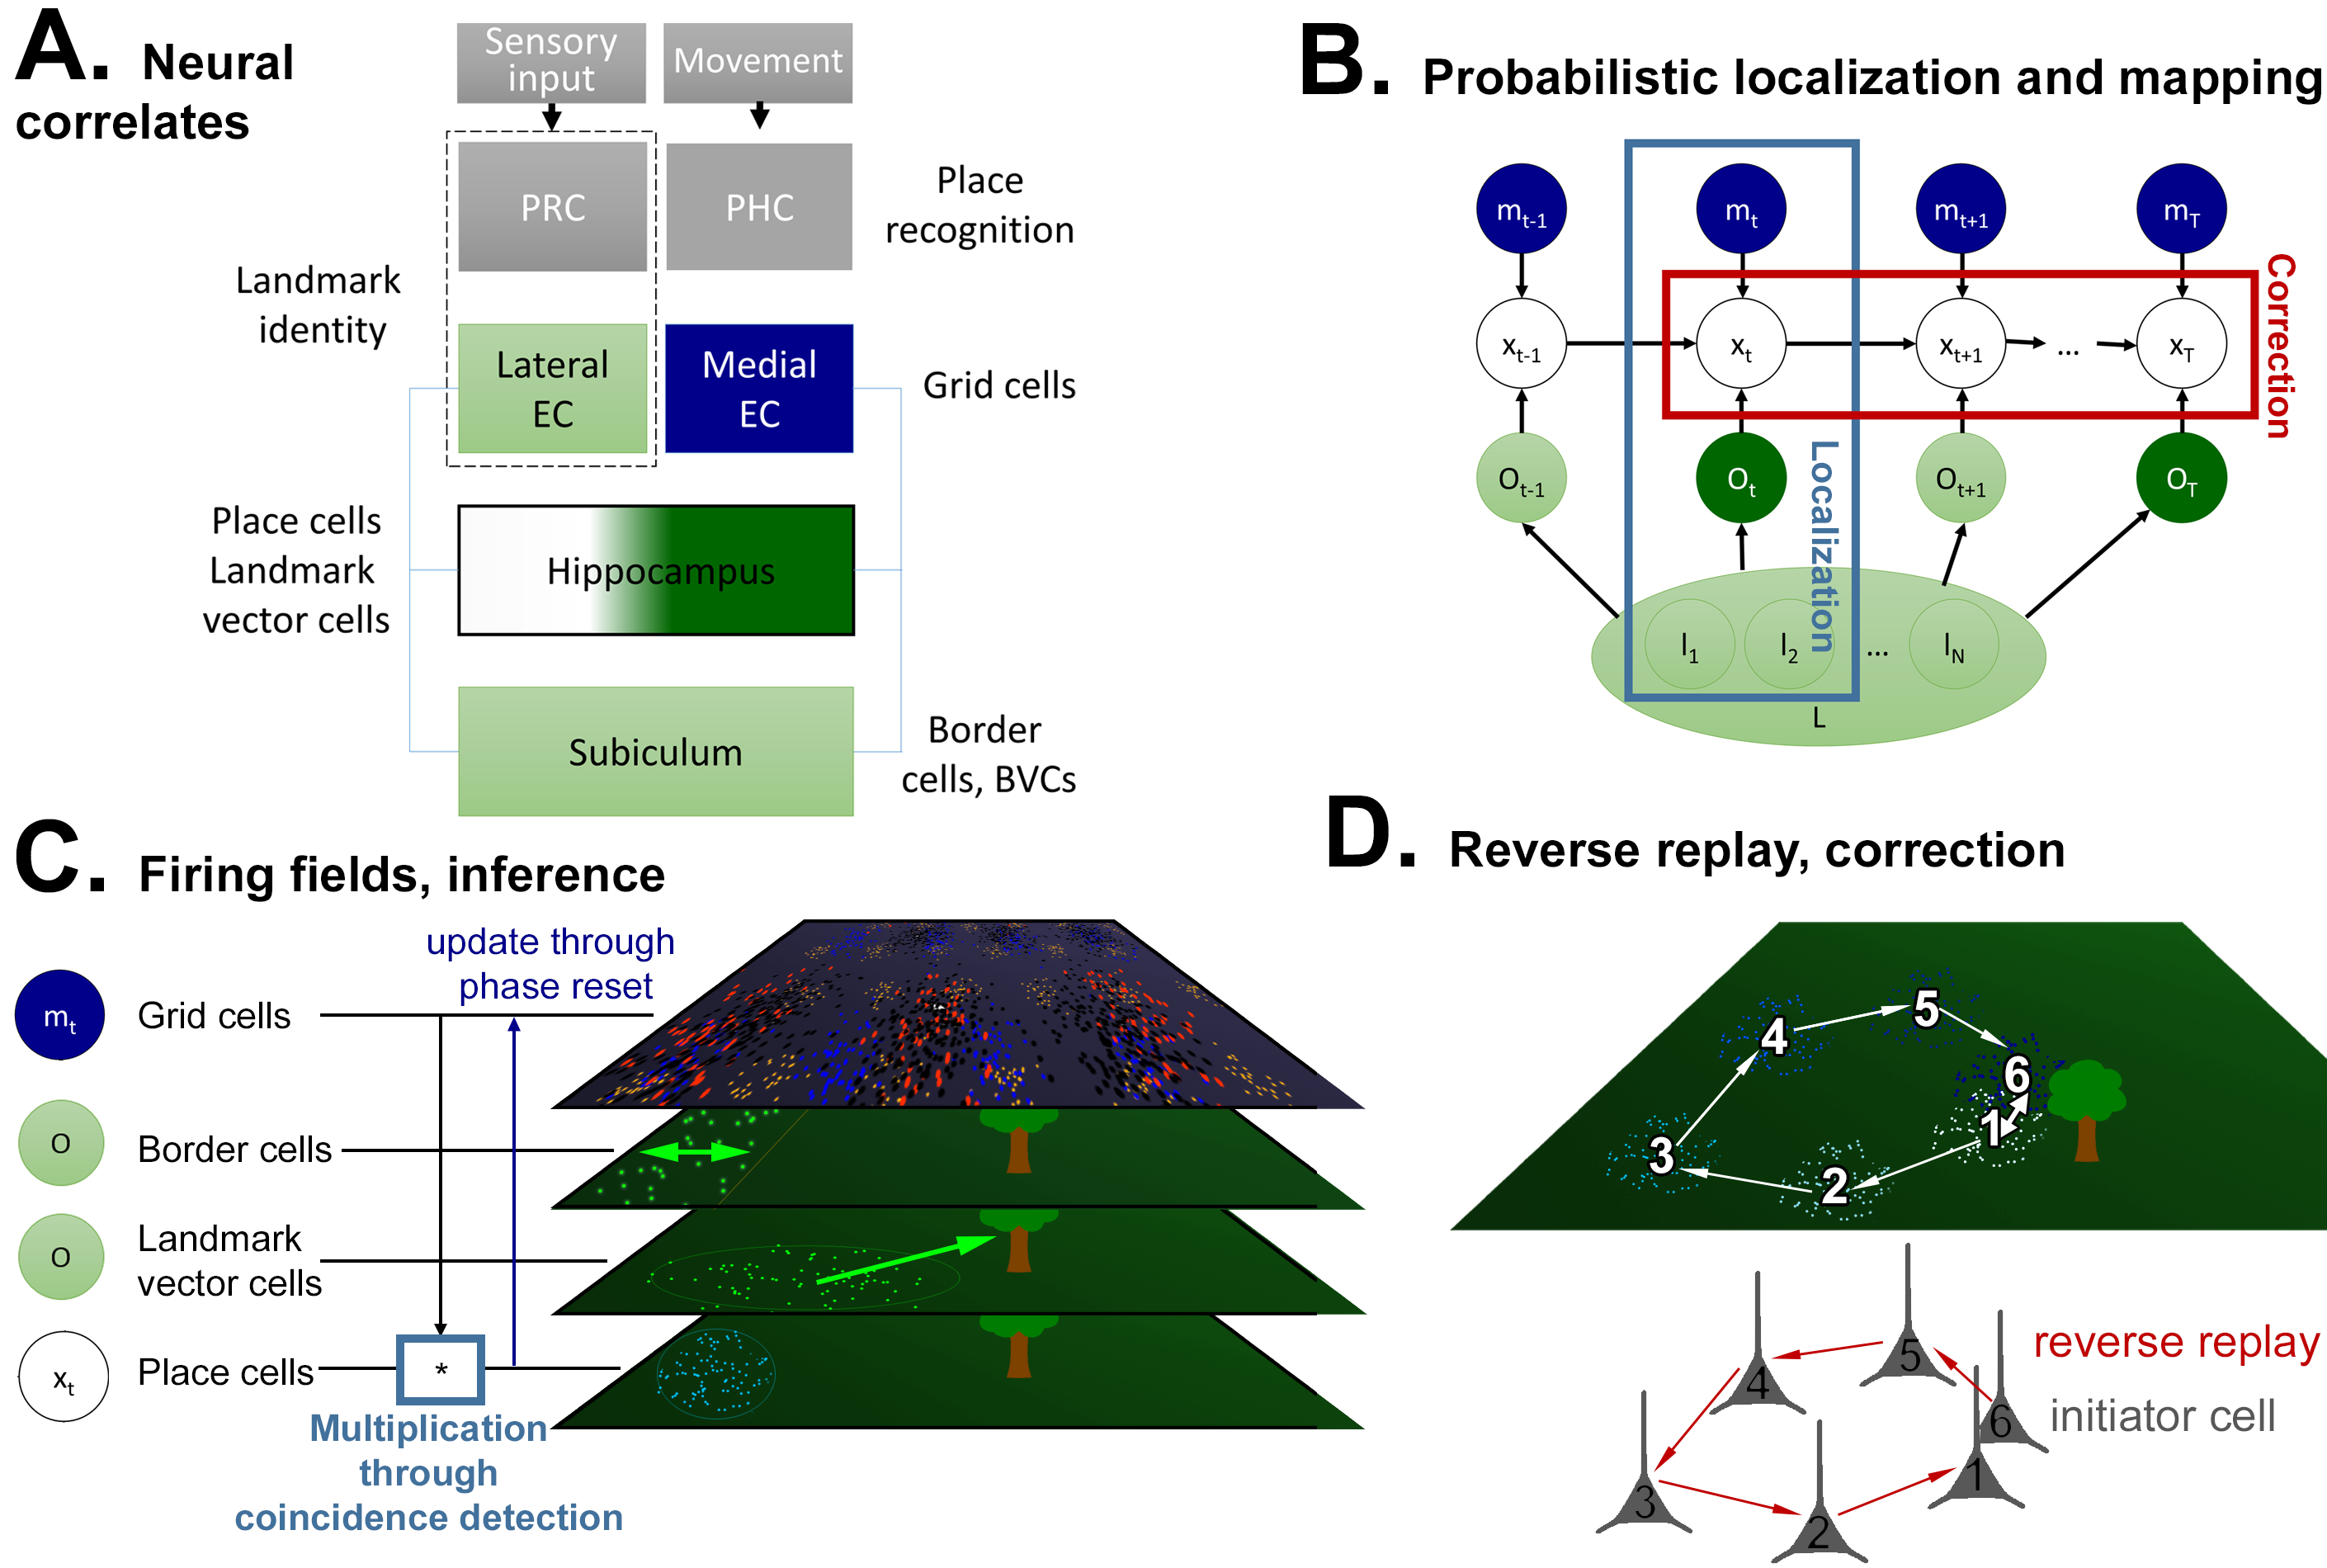
\includegraphics[width=\textwidth]{img/neurimpl3}
	\caption[Probabilistic spatial localization and mapping implementable by brains]{\textbf{Probabilistic spatial localization and mapping implementable by brains}. A: Neural correlates of localization. PRC: Perirhinal cortex, PHC: Parahippocampal cortex, EC: Entorhinal cortex (see Chapter \ref{cha:nnreview} for details; and (Deshmukh et al., 2013) for evidence of landmark vector cells). B: Probabilistic graphical model of the simultaneous localization and mapping problem \citep{thrun2008simultaneous}. Instead of capturing all correlations introduced through the landmarks, which requires vast computational resources, our model separately solves Bayesian localization with only local landmarks, and map correction (`pose optimization' in SLAM) with only loop closure constraints. See Chapter \ref{cha:methods} for notation and details. C: Illustration of firing fields during localization. Coloured dots represent spikes of the respective cells at specific locations. Path integration (grid cells) and boundary and landmark information (border cells, landmark vector cells) is integrated in place cells, using coincidence detection (rejection sampling) to obtain a near-optimal location estimate. This new estimate is used to update grid cell representations via phase reset to combat accumulating path integration errors (see Chapter \ref{cha:bayespc}). D: Illustration of a small loop (firing fields 1-6) which can be corrected upon recognizing the same landmark at positions 1 and 6 via reverse replay, by reactivating place cells 6-1 and shifting their place fields proportionally (see Chapter \ref{cha:lida}).
	} 
	\label{fig:neurimpl}
\end{figure}

\clearpage

\noindent that human spatial memories in particular are organized hierarchically \citep{hirtle1985evidence, mcnamara1989subjective, greenauer2010micro}, but the principles underlying these structures have not been known. We suggest a Bayesian nonparametric clustering model for structuring object representations under a subject-specific metric to account for human cognitive map structure (Section \ref{sec:bayesmap}), and present empirical evidence for this claim gathered from virtual reality and real world environments in Chapter \ref{cha:structure}.




These probabilistic models for inferring self locations and object locations and structuring their representations constitute the pillars of a cognitive software agent able to function in a realistic robotic simulator, which provides the same interfaces as a real robot (and would allow this agent to run on a real robot without modifications to its code) \citep{rusu2007extending}. We have implemented this agent within the LIDA (Learning Intelligent Distribution Agent) cognitive architecture, extending it with a spatial memory module and the described probabilistic models, integrating them with the other mechanisms already implemented in LIDA. Describing LIDA is outside the scope of this thesis, but see the review by \cite{franklin2013lida}, co-authored during this PhD.

Figure \ref{fig:neurimpl} above provides an overview over how the Bayesian mechanisms summarized above may be implemented in spatially relevant brain areas, and pointers to the parts of this thesis substantiating these connections; lending credence to our claim that our probabilistic models are neurally plausible (implementable in brains). Chapter \ref{cha:bayespc} provides the first neural-level evidence for Bayesian inference in these brain areas. 
%The rest of this thesis is concerned with showing that these mechanisms are useful in modelling human behaviour, and in making cognitive models work on robots.

%More specific and detailed descriptions of each method, including the empirical methods used to gather data for testing hypotheses for which no existing datasets could be found, are described in the respective result chapters. Chapter \ref{cha:bayespc} contains descriptions of the place cell firing data and its computational modelling, and Chapter \ref{cha:structure} the collection of data regarding spatial memory structure and accuracy data and its modelling. Chapter \ref{cha:lida} integrates the models in the same architecture, and interfaces them to a robotic simulator. 

%Describing the details of the LIDA (Learning Intelligent Distribution Agent) cognitive architecture \citep{franklin2013lida}, within which these cognitively plausible Bayesian mechanisms have been computationally realized, is outside the scope of this thesis.


\section{Probabilistic modelling}

Probabilistic models use probability distributions to represent quantities and the uncertainties associated with them, utilizing probability theory to manipulate these distributions \citep{ghahramani2015probabilistic}. Two basic rules provide the foundation, and together yield Bayes' theorem, which underlies Bayesian modelling. The \textit{sum rule} takes the form

\begin{equation}
\label{sumrule}
p(Y) = \sum_{X} p(Y, X),
\end{equation}

where $p(X,Y)$ is the joint probability of random events X and Y both happening, and the summation is over all values which $Y$ could possibly take. $p(X)$ is also referred to as the marginal probability, and the summation in Equation \ref{sumrule} is also called marginalization (which is especially useful to make inferences about variables of interest by summing out all other variables). The \textit{product rule} states that

\begin{equation}
\label{productrule}
p(Y,X) = p(Y|X)p(X) = p(X|Y)p(Y),
\end{equation}

\noindent where $p(Y|X)$ is the conditional probability (i.e. the probability of Y given X). Combined, they yield \textit{Bayes' theorem}:

\begin{equation}
\label{bayesrule}
p(Y|X) = \frac{p(X|Y)p(Y)}{p(X)} = \frac{p(X|Y)p(Y)}{\sum_{Y} p(X, Y)}.
\end{equation}

In the context of a probabilistic model, defined by a number of parameters encoded in $Y$ (such as the current coordinates of an agents location), and given some observed data encoded in $X$ (such as the distances to landmarks), we can use Equation \ref{bayesrule} to calculate a \textit{posterior} probability distribution of model parameters, combining \textit{prior} knowledge (or assumptions) $p(Y)$ with the \textit{likelihood} $p(X|Y)$.

The sections below summarize computational-level solutions to the problems required for real-world spatial cognition outlined in Chapter \ref{cha:intro} in this probabilistic framework. As mentioned there, the goal of this work is contributing to the understanding of spatial information processing in brains and minds, and not finding particularly accurate solutions to these problems. Numerous algorithms capable of much more accurate localization and mapping and making less restrictive assumptions have been proposed in probabilistic robotics \citep{thrun2005probabilistic}, more specifically simultaneous localization and mapping (SLAM) - see \citep{thrun2008simultaneous,durrant2006simultaneous,bailey2006simultaneous} for reviews and \citep{tuna2012evaluations} for a more recent evaluation. 

Our particular computational-level solutions for estimating locations utilize stronger simplifications compared to the state of the art in SLAM. We are applying existing computational and mathematical tools to cognitive and neural mechanisms, following a long and successful history of this approach in the field of computational cognitive modelling \citep{sun2008introduction}, which can be seen as a branch of applied computer science. In this field, simplicity and approximations can be assets; since humans are unlikely to use computationally complex, optimal statistical models (see e.g. \citep{van2008tractable,simon1955behavioral}). A simpler, sub-optimal model which nevertheless explains empirical data better, and is more consistent with neural anatomy, is better suited to modelling cognition than an intractable or implausible optimal model. The implementation of these abstract methods in a way consistent with the neuroscience and psychology of spatial memory is novel, as is their integration with a comprehensive cognitive architecture and their substantiation with empirical data (see Section \ref{sec:intro:outline} for the full list of novel contributions). 

\section{Bayesian cue integration}
\label{sec:bayescue}

One concrete application of Equation \ref{bayesrule} is the inference of the most likely current location of an animal, given some observations regarding the distance of a number of landmarks. For simplicity, we assume 1) a uniform prior over these observations, and 2) conditional independence of the observations given the location. The posterior probability of the current location $p(\bm x | O)$, given a location prior $p(\bm x)$ and some observations $\bm o_1, ..., \bm o_N \in O$ (and a normalization constant $\gamma$), is 

\begin{equation}\label{bayes1}
p( \bm x | O ) = \frac{p( \bm x ) p( O | \bm x )}{p(O)} = \gamma p( \bm x ) p( O | \bm x )
\end{equation}

The prior can be obtained by adding up self-motion signals (a process called `path integration' or dead reckoning - see Chapter \ref{cha:nnreview}). Individual observation distributions can express distance measurements to landmarks, and can be multiplied due to their conditional independence given the location:

\begin{equation}\label{bayes2}
p( \bm x | O ) = \gamma p( \bm x ) \prod_{i=1}^{N} p( O_i | \bm x ).
\end{equation}

For now, we further assume that each of these variables is normally distributed. We will use this simplified formulation to predict the sizes of place cell firing field in Chapter \ref{cha:bayespc}; but will implement our localization model without this restrictive assumption, based on rejection sampling (see next section - if all types of noise were Gaussian, the formulations would be functionally equivalent, but the sampling model performs better if this is not the case). The Gaussian assumption makes it straightforward to derive the variance $S_L$ of the normal/Gaussian posterior location distribution $p( \bm x | O ) = \mathcal{N}(\bm x ; \mu_L, S_L)$ from the variances of the prior and of the likelihood distributions $S_x$ and $S_{o,i}$ (see e.g. \cite{wu2004properties} for the derivation of the parameters of products of Gaussian distributions):

\begin{equation}\label{bayes3}
S_{P}=(S_x^{-1}+\sum_{i=1}^{N} S_{o,i}^{-1})^{-1}.
\end{equation}

In the one-dimensional case, the variance is the square of the standard deviation $\sigma$. We can say that the standard deviation of a Gaussian distribution is a measure of the `uncertainty' associated with it (as it measures the spread among possible values - the more certainly a value is known, the lower the associated $\sigma$ of the distribution describing it). Assuming that the observation uncertainties $\sigma_{o,i}$ depend linearly on the respective distances $d_{i}$, such that $\sigma_{o,i}=s \cdot d_{i}$ (Chapter \ref{cha:bayespc} provides justifications and evidence for this linear relationship), we obtain the standard deviation of the location posterior for a given set of measurement distances:

\begin{equation}\label{bayes4}
\sigma_{P}(d_1, ..., d_N)=\sqrt{(\sigma_x^{-2}+s \sum_{i=1}^{N} d_{i}^{-2})^{-1}}.
\end{equation}

Chapter \ref{cha:bayespc} uses Equation \ref{bayes4} to test the hypotheses that place cells may represent uncertainty and perform Bayesian cue integration. Although place cells constitute a two-dimensional representation, this one-dimensional treatment of observation likelihoods is an acceptable approximation in the kinds of environments from which the data was collected (rectangular boxes without landmarks, where the axes can be assumed to be independent as they are orthogonal, and a very narrow, circular track with landmarks, where the width can be neglected as it is less than $3\%$ of the length). 



%Figure \ref{fig:bayescue}

%\begin{table*}[h]
%	\centering
%	{\renewcommand{\arraystretch}{1.2}
%		\begin{tabu}{c|c}
%			$\downarrow$ {Dimensions} & {Variance of the location posterior}\\ \tabucline[3pt]{-}
%			1D & $\sigma^2_{L1D}=(\frac{1}{\sigma_x^2}+\sum_{i=1}^{N} \frac{1}{\sigma_{o,i}^2})^{-1}$ \\
%			2D & $S_{L2D}=(S_x^{-1}+\sum_{i=1}^{N} S_{o,i}^{-1})^{-1}$ \\
%		\end{tabu}
%	}
%	\caption[Variance of the posterior location estimate under Gaussian assumptions]{\textbf{Variance of the posterior location estimate under Gaussian assumptions}. $\sigma$ stands for scalar standard deviations, and $C \in \mathbb{R}^{2x2}$ for covariance matrices.}
%	\label{tbl:bayescue}
%\end{table*}

\begin{figure}[h]
	\centering
	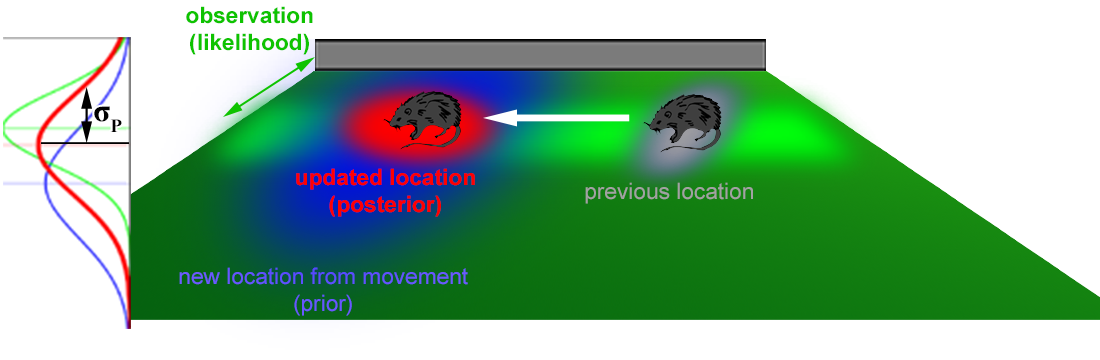
\includegraphics[width=\textwidth]{img/bayesian_localization3}
	\caption[Bayesian cue integration for localization]{\textbf{Bayesian cue integration for localization.} Illustration of how an animal might use its prior location belief (blue) estimated from its movement, and distance distributions e.g. to a boundary (green) to obtain a corrected location estimate (red) using Bayesian inference.} 
	\label{fig:bayescue} 
\end{figure}

%
\section{Bayesian localization}
\label{sec:bayesloc}

To maintain a location estimate through time, the kind of cue integration described above has to be performed regularly (after every time step). One source of location information is adding up each movement vector, a process called odometry in robotics and `path integration' in cognitive science and biology. However, movements are not accurate and noise free in real-world environments - each movement vector contains a slight error, and these errors add up over time. Eventually, these accumulating errors render the location estimate useless, if sensory information is not used to correct it. 

Bayesian localization is concerned with correcting the location estimate in time using noisy observations \citep{thrun2005probabilistic}. Conceptually, it entails performing the Bayesian cue integration to correct location estimates \textit{recursively}, after every movement / time step. Its operation can be summarized in three stages, which are performed iteratively at every time step: 1) movement (adding the current movement), 2) correction of the location estimate via Bayesian cue integration, 3) updating of the path integration estimate for use in the next iteration.

Unlike the simplified treatment above, which has considered only one snapshot in time, Bayesian localization considers the posterior at any time step $t$. This posterior distribution has to depend on all movements until now: $\bm m_{1:t}$, on all observations until now: $ O_{1:t}$, as well as the locations of known landmarks $\bm l_{1:N}$. Extended by these dependencies, the posterior location distribution from Equation \ref{bayes1} becomes

%specifying the probability distribution of the current position $ x_{t} $ given motor commands $u$, measurements $z$, and landmarks $l$. This expression can be expanded using Bayes' rule,

\begin{equation}
\label{bayesloc1}
p(\bm x_{t} | \bm m_{1:t}, O_{1:t}, \bm l_{1:N}) = \gamma p(O_{t} | \bm x_{t}, \bm l_{1:N}) p(\bm x_{t} | \bm m_{1:t}),
\end{equation}

\noindent through simple application of Bayes' theorem. We can use the sum rule (with the sum replaced by an integral for dealing with continuous distributions) to model the `path integration' (odometry) mechanism which provides the prior in Equation \ref{bayesloc1}:

\begin{equation}
\label{prior}
p(\bm x_{t} | \bm m_{1:t}) = \int p(\bm x_{t} | \bm x_{t-1}, \bm m_{t-1}) p(\bm x_{t-1} | \bm m_{1:t-1}) \mathrm{d} \bm x_{t-1}.
\end{equation}

This equation allows inferring the current location prior based on the most recent movement $\bm m_{t-1}$ and on the previous location estimate $\bm x_{t-1}$ by marginalizing (integrating out) the previous location. This is a recursive formulation which yields a path integration estimate based on a starting location and a number of movements. This estimate is subject to accumulating errors. However, crucially, the corrected previous location estimate (previous posterior) can be used instead of the uncorrected previous path integration estimate. Using this insight, replacing $p(\bm x_{t-1} | \bm m_{1:t-1})$ in Equation \ref{prior} by the previous location posterior $p(\bm x_{t-1} | \bm m_{1:t-1}, O_{1:t-1}, \bm l_{1:N})$ and plugging the resulting prior into Equation \ref{bayesloc1} yields

\begin{equation}
\label{bayeslocsolution}
\begin{split}
p(\bm x_{t} | \bm m_{1:t}, O_{1:t}, \bm l_{1:N}) = \gamma p(O_{t} | \bm x_{t}, \bm l_{1:N}) \int p(\bm x_{t} | \bm x_{t-1}, \bm m_{t-1}) \cdot \\
 p(\bm x_{t-1} | \bm m_{1:t-1}, O_{1:t-1}, \bm l_{1:N}) \mathrm{d} \bm x_{t-1}
\end{split}
\end{equation}

This recursive equation for updating location estimates is a Bayes-optimal solution to the localization problem and allows inferring the current location based on two conditional densities: a model specifying the effect of movements on the location (a `motion model'):
\begin{equation}\label{motionmodelq}
p(\bm x_{t} | \bm x_{t-1}, \bm m_{t-1})
\end{equation}
and a model specifying the probability distribution of the current measurements $ O_{t} $ at a position $ \bm x_{t} $ given the landmarks $ \bm l_{1:N} $ (a `sensor model'):
\begin{equation}\label{sensormodelq}
p(O_{t} | \bm x_{t}, \bm l_{1:N}).
\end{equation}

Equation \ref{bayeslocsolution} is the mathematical formulation of Bayesian localization, which, conceptually, iterates over the three stages mentioned above: movement (application of the motion model), correction (via Bayes' theorem), and update.

As argued in Chapter \ref{cha:bayespc} and Appendix \ref{apx:bayespc}, the activity of hippocampal place cells can be viewed as samples from probability distributions, and the size of their firing fields can be partially predicted by a Bayesian model. We will also argue based on existing evidence that the `motion model' is implemented by a neural path integrator in the entorhinal cortex, and that neurons with boundary-related firing might implement the `sensor model'.

Such a sampling-based representation of uncertainty in these spatially relevant brain areas naturally suggests employing a sequential Monte Carlo method \citep{doucet2000sequential} to computationally evaluate the integral in Equation \ref{bayeslocsolution} (the same model using samples for representation might as well use them for inference). Although the usual method of choice in robotics is importance sampling \citep{montemerlo2007fastslam, thrun2005probabilistic}, we approximate the integral using rejection sampling \citep{doucet2000sequential}, and will argue in Chapter \ref{cha:bayespc} and Appendix \ref{apx:bayespc} that coincidence detection (CD) in hippocampal place cells can implement this mechanism (since CD can filter out samples at locations where different measurements and path integration disagree, and keeps the ones where they agree - see illustration in Figure \ref{fig:neurimpl}C, and Appendix \ref{apx:bayespc} for mathematical details). 

From a computational point of view, instead of inferring the parameters of the location posterior distribution (e.g. the mean and variance in case of a Gaussian), we represent it by sampling multiple location hypotheses. The mean of these hypotheses corresponds to the 'best guess' estimate, and their standard deviation to the associated uncertainty. Apart from the empirical evidence for sampling based mechanisms in the brain (see Chapter \ref{cha:bayespc}, as well as \citep{fiser2010statistically} for a more general review), the main advantage of this approach is the ability to represent free-form distributions (irregular, non-Gaussian, multimodal distributions etc.).

Particles (samples, hypotheses) $\bm x^i$ are generated regularly based on self-motion information (linear and angular movement speed $v$) according to the motion model (Equation \ref{motionmodelq}), performing path integration at simulated timesteps $ \Delta t $. In the simplest case: $ \bm x_{t}^i = \overline{\bm x}_{t-1} + \bm m_t $, with $\bm m_t=T(\bm v'\Delta t)$, and $T$ simply transforming from polar (linear and angular speed) to Cartesian coordinates. Gaussian noise is multiplied to the estimated speed to obtain a distribution of hypotheses reflecting the path integration / odometry uncertainty (neither animals nor robots can estimate their movement speed with perfect accuracy):

\begin{equation}\label{veq}
\bm v' = \bm v_{true} \cdot \mathcal{N}(\bm 1, \begin{bmatrix}\sigma_v^2 & 0\\ 0 & \sigma_\omega^2\end{bmatrix})
\end{equation}

\noindent where $ \sigma_v^2 $ and $ \sigma_\omega^2 $ are model parameters representing the variance in the linear and angular speeds, respectively. Since the estimate of $\bm v$ is noisy, accumulating errors would lead to an increase of uncertainty and the corruption of the distribution represented by the set of particles, which is why correction with the sensor model is required. 

Under Gaussian assumptions, this correction can be implemented simply by multiplying a path integration prior and a number of sensory likelihoods and solving for the means and variances (Equation \ref{bayes2}). The ensuing algorithm for Bayesian localization is trivial. When using samples instead of a Gaussian to represent the posterior, the correction can be implemented by rejection sampling \citep{doucet2000sequential}, i.e. by deleting hypotheses inconsistent with sensory measurements (see Figure \ref{fig:bayesloc}). The derivation of why this rejection sampling scheme approximates the true Bayesian posterior can be found in Appendix \ref{apx:bayespc}. Details regarding how brains could implement this algorithm are discussed in Chapter \ref{cha:bayespc}.

\begin{figure}[h]
	\begin{pseudocode}{movement}{samples, \textbf{v}, N}
		1: prevmean \GETS mean(samples) \\
		2: newsamples \GETS \{ \} \\
		3: \FOREACH particle \in samples \\
		4: \quad newsamples \GETS newsamples \cup \{motionModel(particle, \textbf{v})\} \\
		5: \WHILE count(newsamples) < N \\
		6: \quad newsamples \GETS newsamples \cup \{motionModel(prevmean, \textbf{v})\} \\
		7: return(newsamples)
	\end{pseudocode}
	\begin{pseudocode}{correction}{samples, \textbf{O}, \textbf{L}}
		1: newsamples \GETS \{ \} \\
		2: \FOREACH particle \in samples \\
		3: \quad likelihood \GETS sensorModel(particle, \textbf{O}, \textbf{L}) \\
		4: \quad \IF random() < likelihood \\
		5: \quad \quad newsamples \GETS newsamples \cup \{particle\} \\
		6: return(newsamples)
	\end{pseudocode}
	\begin{pseudocode}{localizationStep}{posteriorsamples, \textbf{v}, \textbf{O}, \textbf{L}, N}
		1: timestep++ \\
		2: movedsamples \GETS movement(posteriorsamples, \textbf{v}, N) \\
		3: correctedsamples \GETS  correction(movedsamples, \textbf{O}, \textbf{L}) \\
		4: return(correctedsamples)
	\end{pseudocode}
	\centering
	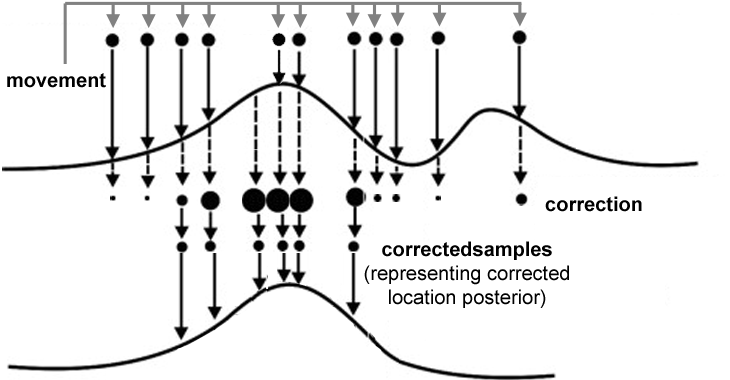
\includegraphics[width=0.75\textwidth]{img/rejectionsampling}
	\caption[Bayesian localization algorithm with rejection sampling]{\textbf{Bayesian localization algorithm with rejection sampling,} producing updated posterior samples given the samples from the previous posterior, speed vector $\bm v$ and observations $O$ at the current time step, landmarks $L$, and a particle budget $N$}
	\label{fig:bayesloc}
\end{figure}

%To correct this distribution, and to estimate the target posterior distribution \eqref{bayeslocsolution}, each particle is weighted according to the likelihood of the perceived sensory measurements from the location hypothesis represented by the particle, i.e. according to the sensor model: 
%$\bm w_t^i=p(O_t|\bm x_t^i, O_{t-1}, \bm m_t)$. This approach of estimating a target distribution is called importance sampling (see e.g. \cite{montemerlo2007fastslam, thrun2005probabilistic} for the derivation).

\clearpage

\section{Maximum likelihood map error correction}
\label{sec:bayescorr}

Landmark location estimates can be updated in the same way as the agents' location estimates $\bm x$, by integrating new observations into the posterior distribution representing these locations (either in the form of Gaussians or of samples from this distribution). With infinitely many particles, the algorithm presented in Figure \ref{fig:bayesloc} would suffice to maintain correct location estimates. 

However, there are practical limits on the particle budget (due to limited computational resources in computers, and due to limited firing rates in neurons). This necessarily leads to errors whenever there is no particle at the unobservable true location. Unfortunately, these errors add up as well. They become most pronounced when revisiting an already known part of the environment, i.e. when traversing a loop - although the agent has returned to its starting location, it will think that it is at a new location, and form new representations of the same place. Multiple such loops can lead to multiple redundant, erroneous representations. 

The problem of how to correct spatial representations when revisiting a known place (not only the location estimate but also the estimated recent path and landmark locations) is the `loop closing' problem in robotics (see e.g. \citep{williams2009comparison, thrun2008simultaneous}). Brains need to solve this problem as well - although human spatial representations are not perfectly accurate, humans are able to correct mistaken estimates when they recognize a revisited place. Interestingly, despite the abundant robotics literature on the topic of closing loops, this problem has been largely neglected in cognitive science literature. 

Our cognitive model of loop closing is described in more detail Chapter \ref{cha:lida}. Here, we will briefly summarize its purely computational and mathematical aspects. We will assume that it is sufficient to correct the route taken during the loop, i.e. the most recent locations of the agent; and that the landmarks are corrected by the same amount as the location closest to them. That is, when performing large-scale loop closing, the model in Chapter \ref{cha:lida} applies the same correction to a position and the local landmarks around it (a simplification justified based on neuroscientific evidence in that Chapter). We also make the assumption that correction only concerns position representations and not angular representations, once again based on neural evidence. Hippocampal `reverse replay' \citep{carr2011hippocampal} (the re-activation of recently active place cells) is a plausible mechanism for correcting the recent route when revisiting a location, as argued in Chapter \ref{cha:lida}, but such a mechanism has not been found for neurons with direction-specific firing.

When revisiting a known place, the recently traversed path has to be corrected using the discrepancy between the previously and recently estimated location of the revisited place. Naturally, when an agent recognizes that it is in the same place it has visited before, the current estimate has to be reset to be equivalent to the previous estimate of the same location. However, it is not obvious how to correct the other recently visited locations $\bm x_0, ..., \bm x_m \in X$ along the recent path $X$. Let $\bm c_1, ... \bm c_m \in C$ denote a set of vectors we will call constraints, each expressing how far apart two locations should be according to some measurement. That is, each constraint specifies the difference between two locations $\bm c=\bm x_a-\bm x_b$, and each is associated with a measurement uncertainty $S_c$ in the form of the covariance matrix of a normal distribution. For locations traversed in sequence, $\bm c$ and $S_c$ is given by the motion model (by path integration). For revisited locations, $\bm c$ is zero (there should be no difference between the location estimated when encountering that place first and when revisiting it). 

According to Bayes' theorem, and assuming that constraints are independent given the locations, the recent path depends on the product of the constraint distributions; and the best path estimate is the one that maximizes:

\begin{equation}
\label{loopprob}
P(X|C) \propto \prod_{i=1}^{m} P(\bm c_i|X) 
\end{equation}

Each $P(\bm c_i|X)$ expresses the likelihood that this constraint is satisfied by the path $X$, as a Gaussian distribution: $P(\bm c_i|X)\propto\mathcal{N}(\bm x_a-\bm x_b;\bm c_i, S_i)$ (where $\bm x_a$ and $\bm x_b$ are the location estimates which should have the distance $\bm c_i$ according to this constraint). We are interested in the maximum of Equation \ref{loopprob}, which is equivalent to the minimum of its negative logarithm. Let $\bm d_i=\bm x_a - \bm x_b - \bm c_i$ be the discrepancy between the constraint and the locations it concerns within the path. With noise-free measurements, all $d_i$ would be zero; but since sensory errors may add up, there will be discrepancies (e.g. after traversing a loop, the estimate of the first visit $\bm x_a$ and second visit $\bm x_b$ may differ, but $\bm c_i=0$ for the revisited place). Then, the most likely path is given by:

\begin{equation}
\label{mleq}
X_{ml} = \argmax_X P(X|C) = \argmin_X -log P(X|C) = \argmin_X \sum_{i=1}^{m} ||\bm d_i||_{S_i^{-1}}.
\end{equation}

Equation \ref{mleq} mathematically describes the maximum likelihood error correction problem for loop closing. It tries to minimize the discrepancies between the constraints and the estimated locations, taking into account the constraint uncertainties $S_i$ by utilizing the Mahalanobis distance\footnote{The Mahalanobis distance is defined as $||\bm x_1-\bm x_2||_S = \sqrt{(\bm x_1-\bm x_2)^TS(\bm x_1-\bm x_2)}$} to measure the discrepancy.

There are several ways to solve Equation \ref{mleq}. For our cognitive model (Chapter \ref{cha:lida}), we chose sequential gradient descent, because it can be implemented in biological neurons \citep{bengio2015towards, bengio2015objective}. \cite{olson2006fast} derive the starting point for this solution. They suggest the following gradient with respect to constraint $i$, depending on a learning rate $\alpha$, a full Jacobian $J$ of the constraints with respect to the path, and the Jacobian $J_i$ of constraint $i$:

\begin{equation}
\label{gradient}
\Delta X \approx \alpha (JS^{-1}J)^{-1}J_i^TS_i^{-1} \bm d_i.
\end{equation}

Because of the incremental structure of the Jacobian, it is possible to simplify this expression (see Chapter \ref{cha:lida}). Making use of this structure, and defining a loop precision parameter $A_i=S_i/S_P$ specifying the ratio of the uncertainties of loop closure constraints (added when revisiting a place) and path integration constraints, the gradient for each individual location within the loop becomes:

\begin{equation}
\label{correction}
\Delta \bm x_j \approx \alpha d_i \frac{\sum_{k=a+1}^{j} S_i^{-1}}{\sum_{k=a+1}^{min(j,b)} S_P^{-1}} = \alpha A_i \bm d_i p_j,
\end{equation}

\noindent where $p_j=(min(j,b_i)-a_i-1)/(b_i-a_i-1)$ denotes how far $x_j$ lies along the loop, with $0 \leq p_j \leq 1$. Unlike usual gradient descent procedures, in this particular case we know that $\Delta \bm x \leq \bm d_i $ must hold, and can prevent the algorithm from overshooting, accelerating its convergence. Figure \ref{fig:sgdslam} contains the algorithm using this gradient to correct location estimates when revisiting a place. We will use this algorithm in Chapter \ref{cha:lida} to account for human cognitive map accuracy, as a part of a cognitive architecture embodied on a robot and learning maps in realistic simulated environments.

\begin{figure}[h]
	\begin{pseudocode}{correctPath}{X, loopConstraints, \alpha, A, N}
		1: \WHILE i < N \AND \NOT converged \\
		2: \quad i++ \\
		3: \quad \FOREACH a,b \in loopConstraints \\
		4: \quad \quad discrepancy \GETS X_a - X_b \\
		5: \quad \quad \FOREACH j \in (a,b] \\
		6: \quad \quad \quad p \GETS (min(j,b)-a-1)/(b-a-1) \\
		7: \quad \quad \quad \beta \GETS min(\alpha A \cdot discrepancy, discrepancy) \\
		8:\quad\quad\quad X_j \GETS X_j + \beta p \\
		9: return(X)
	\end{pseudocode}
	\caption[Algorithm for correcting location estimates when revisiting places]{\textbf{Algorithm for correcting location estimates when revisiting places (`loop closing'),} producing a corrected path given the estimates of locations $X$ along that path (from Bayesian localization), a list of loop constraints indicating the same (revisited) places (from landmark recognition or place recognition), a learning rate $\alpha$, a loop precision parameter $A$ and an iteration budget $N$}
	\label{fig:sgdslam}
\end{figure}

\section{Bayesian nonparametrics for map structuring}
\label{sec:bayesmap}

It has been suggested that map-like spatial representations are structured hierarchically \citep{hirtle1985evidence,mcnamara1989subjective,greenauer2010micro}, but no formal model has been put forth for a process that might account for this structure. We hypothesize in Chapter \ref{cha:structure} that this process might be clustering. Computationally, we chose a Dirichlet Process Gaussian Mixture Model (DP-GMM) to account for the behaviour data we collected (see Chapter \ref{cha:structure}), for two reasons. First, DP-GMMs (unlike most clustering algorithms) are able to infer the number of clusters, not just cluster memberships; and are infinitely extensible \citep{rasmussen1999infinite}. Second, Bayesian nonparametric models with Dirichlet priors have a successful history in psychological modelling, e.g. of category learning and causal learning \citep{tenenbaum2011grow}, transfer learning \citep{canini2010modeling}, and human semi-supervised learning \citep{gibson2013human}.

By `map structure', here and in Chapter \ref{cha:structure}, we mean sub-map memberships. There is evidence that human spatial maps are hierarchical \citep{hirtle1985evidence,mcnamara1989subjective,greenauer2010micro}, just as geographical maps are - e.g. there is a map of the country and a map of the cities therein; and any given building may be represented not only on the country map but also on one of the city maps. Similarly, any object (e.g. building) memorized by a participant belongs to her map-like spatial representation (`cognitive map'), as well as to one of its sub-maps. We only consider a two-level hierarchy (map and sub-maps); thus, sub-map memberships fully describe our modelled map structure.

A number of features can influence spatial representation structure, including spatial distance and visual and functional similarity of landmarks. The importance of these features varies across participants, and these subject-specific importances have to be accounted for before the clustering process. We chose to implement a new metric learning method to do so (see below). Our model of spatial representation structure consists of these two components: a subject-specific metric, expressing the `similarity function' between two buildings, and the DP-GMM model for clustering buildings under this metric.

As noted in the Introduction, unlike the rest of our work, we have not shown what the neural implementation of such a structuring process might look like. Some prior work exists showing the possibility of inference in hierarchical Bayesian models such as the DP-GMM, e.g. \citep{shi2009neural} - see \citep{sanborn2015types} for a review. We have substantiated the psychological plausibility of this model by showing that it can explain and predict human behavior data (Chapter \ref{cha:structure}), and leave the investigation of the biological plausibility of this specific mechanism for future work.

\subsection{Dirichlet Process Gaussian Mixture Models for clustering}

We will only describe the DP-GMM model very briefly, since it is a well-established model and since we did not implement it ourselves in this work (we used the $bnpy$ Python library instead). See e.g. \citep{rasmussen1999infinite} for its introduction, or \citep{gershman2012tutorial} for a tutorial. The DP-GMM partitions a number of data points $x$ into $K$ clusters by fitting a mixture of $K$ Gaussian distributions to the data. It infers the number of clusters, as well as the means $\bm \mu_k$ and covariances $\Sigma_k$ of each Gaussian, by inverting the generative process defined as follows:
 
\begin{equation}
\label{eq:dpgmm}
\begin{array}{rcl}
\phi_k   \sim Beta(1, \alpha_1) \\
\bm \mu_k    \sim Normal(0,  \mathbf{I}) \\
\Sigma_k \sim Wishart(D, \mathbf{I}) \\
\pi_{k}  \sim SBP(\phi) \\
\bm x_t \sim Normal(\bm \mu_{z_i},  \Sigma_{z,i}^{-1}),
\end{array}
\end{equation}

\noindent where SBP stands for the stick-breaking process for generating mixture weights: $\pi_k=v_k \prod_{j=1}^{k-1} (1-v_j)$. Data can be generated from this model by first choosing a cluster with probabilities specified by mixture weights: $z \sim Cat(\pi)$, and then drawing an observation from the parameters of that cluster $\bm x \sim Normal(\bm \mu_z, \Sigma_z)$.

Given the data, the parameters of this model (i.e. the $\bm \mu_z$ and $\Sigma_z$ describing each cluster, and the cluster memberships $z$ of the data points) can be inferred using either a Monte Carlo chain sampling method \citep{neal2000markov} or variational inference \citep{blei2006variational}. We did not implement an inference algorithm in this work; instead, we have used the $bnpy$ Python library for this purpose. See \citep{hughes2013memoized} for implementation details.

\subsection{Metric learning in absolute pairwise difference space}

In order to learn a suitable metric for our data, we had to develop a novel metric learning method, since the assumptions made by existing methods do not hold in our case. Neither the linear separability assumption (made by linear metric learning), nor the prerequisite of roughly isotropic variances along the features (made by RBF-based methods \citep{ong2005learning}) is the case for all subjects in our dataset (see Appendix E for further motivation and evaluation from a machine learning perspective). 

Furthermore, our metric can naturally incorporate the hypothesis that building pairs belonging to the same representation should be located close to the origin in pairwise difference space (i.e. they should not be very different), and should be separable from building pairs belonging to different representations. These two distributions of pair differences can be naturally modelled using Gaussian distributions (\ref{cha:structure}). 

Our proposed method can be seen as a novel approach to perform non-linear metric learning using weak supervision in the form of pairwise constraints, in order to improve clustering performance, as pioneered by \cite{xing2002distance}. The problem to be solved can be defined as follows. Let $\mathcal{X}=(\bm x_i, ..., \bm x_n)$ be the feature vector representation of $n$ objects (buildings on a cognitive map) which are to be clustered (assigned to representations we will call `sub-maps'), where $\bm x_i \in \mathbb{R}^D$ are vectors with $D$ dimensions. Let the set of $m$ given labelled pairwise co-representation constraints be denoted by $\mathcal{C}$, where $ \lvert \mathcal{C} \lvert = m $, and $c_{i,j} \in \mathcal{C}$ is

\begin{equation}
c_{i,j}=
\begin{cases}
1, & \text{if $i$ and $j$ belong to the same sub-map (co-represented)} \\
0, & \text{if $i$ and $j$ belong to different sub-maps (not co-represented)}
\end{cases}
\end{equation}

Our ultimate goal is to group the $n$ objects into $K$ clusters (`sub-maps'), such that objects of the same cluster are more similar to each other than to those of different clusters; taking into account the provided pairwise constraints to learn a good similarity metric for the given data. In our application of this method to spatial representation structure, the pairwise constraints express which pairs of buildings are co-represented in participants' memory, and are obtained from recall sequences (using the assumption that co-represented items are always recalled together) - see Chapter \ref{cha:structure}.

Conventional approaches leveraging non-linear metric learning for this problem try to find a kernel $\Phi$ such that the clustering resulting from using the distance metric defined by that kernel, $d_m^2(\bm x_1, \bm x_2)=(\Phi(\bm x_1)-\Phi(\bm x_2))^T(\Phi(\bm x_1)-\Phi(\bm x_2))$, does not violate the provided constraints (ensures co-represented pairs are closer than other pairs, if possible), and often employ RBF kernels for this purpose, e.g. \citep{baghshah2010kernel, chitta2011approximate}. 

In contrast, the proposed framework aims to learn the distribution of co-representation probabilities (whether or not two object should be linked) from the provided set of constraints, and constructs a pseudo-metric based on a generative model of co-representation probabilities. Crucially, this probabilistic model is defined on the vector space of absolute pairwise differences (APD), which allows learning the importance of each feature (a challenge for RBF kernels for data with non-isotropic variance). Learning in APD space has been proposed before by \cite{zheng2011person} (specifically for person re-identification in computer vision), but not as a general metric learning method. The metric based on this generative model is a pseudo-metric, because it does not satisfy the conditions of subadditivity, $d_m(\bm x, \bm z) \leq d_m(\bm x, \bm y)+d_m(\bm y,\bm z)$ and the identity of discernibles, $d_m(\bm x, \bm y) = 0 \enskip \text{if and only if} \enskip \bm x = \bm y$.

Let $[\Delta \bm{x_{i,j}}]_+ = \big( \lvert \bm{x_{i,k}} - \bm{x_{j,k}} \lvert \big)_{k=1}^m $ be the representation of each pair of objects $(i,j)$ in APD vector space. The co-representation probability distribution, i.e. the posterior probability of any pair of objects belonging to the same cluster, given a pair of objects and some model parameters $\bm{\theta}$ is then 

\begin{equation}
\label{eq:linkprob}
p(c=1|\Delta \bm{x}, \bm{\theta}) \propto p(\Delta \bm{x} | c=1, \bm{\theta}) p(c=1|\bm{\theta})
\end{equation}

The likelihood $ p(c=1|\Delta \bm{x}, \bm{\theta}) $, the model parameters $ \bm{\theta} $ (as well as the prior) can be estimated from $\mathcal{X}$ and $\mathcal{C}$, even in closed form, using Gaussian Discriminant Analysis (GDA). This yields a suitable non-linear pseudo-metric based on this probability distribution - see Equation \ref{eq:metric} -, such that objects likely to belong to the same cluster will be close, and those likely to belong to different clusters will be far apart; with these distances directly depending on co-representation probabilities. 

\begin{equation}
\label{eq:metric}
d_m(\bm x_1, \bm x_2; \bm{\theta}) = 1 - p(c=1|\Delta \bm x, \bm{\theta}) = p(c=0|\Delta \bm x, \bm{\theta})
\end{equation}

A metric is well-suited for clustering if within-cluster instances are closer than across-cluster instances according to it. That is, if for any co-represented $\Delta \bm x_r$ and not co-represented $\Delta \bm x_n $ it holds that $ d_r(\bm x_{r,1}, \bm x_{r,2}; \bm{\theta}) < d_n(\bm x_{n,1}, \bm x_{n,2}; \bm{\theta}) $. It follows from Equation \ref{eq:metric} that this is the case if the generative model learns to separate the absolute differences of within-cluster instance pairs from across-cluster pairs.

In the generative \textbf{GDA} model \citep{bensmail1996regularized}, the likelihoods of a pair of instances either being co-represented (i.e. belonging to the same sub-map), or not being co-represented (i.e. belonging to different sub-maps) are each modelled using a multivariate Gaussian: 

\begin{equation}
\label{eq:mvnormal}
p( \Delta \bm x | c=i; \bm \mu_i, \Sigma_i) = (2\pi)^{-\frac{D}{2}}|\Sigma_i|^{-\frac{1}{2}}\, e^{ -\frac{1}{2}(\Delta \mathbf{x}-\bm\mu_i)^\intercal\Sigma_i^{-1}(\Delta \mathbf{x}-\bm\mu_i) },
\end{equation}

\noindent where $i \in \{0,1\}$. $(\bm \mu_1, \Sigma_1)$ are the means and covariances of the APD distances of co-represented pairs, and $(\bm \mu_0, \Sigma_0)$ those of not co-represented pairs. These parameters can be easily estimated from the given sets of co-represented and not co-represented object pairs, respectively, by calculating their means and covariances. These object pairs (obtained from recall sequences in Chapter \ref{cha:structure}) constitute the training data for the model.

From Equation \ref{eq:mvnormal} and Bayes' theorem, we obtain the posterior probability required for the metric in \ref{eq:metric}, which then becomes:

\begin{equation}
\label{eq:adsgda}
d_m(\bm x_1, \bm x_2; \bm{\theta}) = 1 - \frac{p( \Delta \bm x | c=1; \bm \mu_1, \Sigma_1)}{\sum_{i \in \{0,1\}} {p( \Delta \bm x | c=i; \bm \mu_i, \Sigma_i)}}
\end{equation}

% The crucial difference between Equation \ref{eq:adsgda} and a simple RBF kernel is that the latter can be seen as a symmetric Gaussian `ball' in D-dimensional space, completely described by a single variance parameter. In contrast, the GDA-based model allows implicitly learning the importance of each feature, as well as their covariance, in a non-linear fashion (i.e. it can separate two sets of objects even if they are not linearly separable).

Thus, the trained GDA-model can be used to calculate distances (Equation \ref{eq:adsgda}) between all pairs of objects in any testing data set. The data is projected under the metric in Equation \ref{eq:adsgda} using distance-preserving embedding. We have used multi-dimensional scaling (MDS) for this purpose \citep{borg2005modern}. The result of this projection is a data set embedded such that Euclidean pairwise distances therein, prescribed by Equation \ref{eq:metric}, reflect the structure in the data (close for co-represented and far for not co-represented objects).

We subsequently perform clustering of this resulting data, using a Dirichlet Process Gaussian Mixture Model (DP-GMM) \citep{rasmussen1999infinite}, since the number of clusters is unknown (see previous section). The resulting algorithm for structuring map representations is shown in Figure \ref{fig:structalg}. It requires training data in the form of pairs of co-represented and not co-represented buildings and their features. It allows inferring the metric in closed form and without any hyperparameters that need to be tuned (unlike most metric learning approaches). We use this algorithm to predict the representation structure of participants' cognitive maps in advance in Chapter \ref{cha:structure} (and briefly evaluate its performance on other kinds of data in Appendix \ref{apx:adsmetric}).

\begin{figure}[h]
	\begin{pseudocode}{predictMapStructure}{X, knownX, knownStructure}
		1: corepresented \GETS \{\} \\
		2: notcorepresented \GETS \{\} \\
		3: \FOR i \in (1, |knownX|) \\
		4: \quad \FOR j \in (i+1, |knownX|) \\
		5: \quad \quad \IF knownStructure_i = knownStructure_j \\
		6: \quad \quad \quad corepresented \GETS corepresented \cup (knownX_i-knownX_j) \\
		7: \quad \quad \textbf{else} \\
		8: \quad \quad \quad notcorepresented \GETS notcorepresented \cup (knownX_i-knownX_j) \\
		9: \ \ \mu_{co} \GETS mean(corepresented) \\
		10: \Sigma_{co} \GETS cov(corepresented) \\
		11: coprior \GETS \frac{|corepresented|}{|knownX|} \\
		11: \mu_{not} \GETS mean(notcorepresented) \\
		12: \Sigma_{not} \GETS cov(notcorepresented) \\
		13: notprior \GETS \frac{|notcorepresented|}{|knownX|} \\
		14: D \in \mathbb{R}^{|X|x|X|} \\
		15: \FOR i \in (1, |X|) \\
		16: \quad \FOR j \in (i+1, |X|) \\
		17: \quad \quad D_{i,j} \GETS 1 - \frac{coprior \cdot \mathcal{N}((X_i-X_j); \mu_{co}, \Sigma_{co})}{coprior \cdot \mathcal{N}((X_i-X_j); \mu_{co}, \Sigma_{co}) + notprior \cdot \mathcal{N}((X_i-X_j); \mu_{not}, \Sigma_{not})} \\
		18: embedding \GETS MDS(D) \\
		19: structure \GETS DPGMM(embedding) \\
		20: return(structure)
	\end{pseudocode}
	\caption[Algorithm for predicting spatial representation structure]{\textbf{Algorithm for predicting participants' spatial representation structure}, given the features of the new buildings to be structured, and given buildings with known structure (from a previous experiment) specifying which of these buildings were co-represented.}
	\label{fig:structalg}
\end{figure}

We point out that Equation \ref{eq:metric} constitutes a general framework for metric learning using any model capable of producing probability estimates that two instances belong together. This includes the entire family of generative models in machine learning (see e.g. \citep{bishop2006pattern}), as well as any discriminative model when combined with Platt scaling \citep{platt1999probabilistic} for transforming discrete outputs into probabilities. Constrained clustering is just one application of such a metric - approaches for metric learning have been used for a wide range of tasks including face and activity recognition, text and music analysis, microarray data analysis, etc. \citep{kulis2012metric}. See Appendix \ref{apx:adsmetric} a brief evaluation of the proposed metric on constrained clustering benchmarks.



%\section{Image processing, segmentation, and recognition}

%point out comp aspects WHEREVER POSSIBLE / APPROPRIATE 

%review of methods point out COMP./MATH

%point out what you can get / what you cant get, specifically saying limitations

%limitations 

%\section{Empirical methods}
%
%\subsection{Bayesian localization}
%
%The computational models presented below are based on the hypotheses summarized in Table \ref{tbl:hyp} in the Introduction. Previously gathered and published data was available for testing the hypotheses that hippocampal place cells might encode uncertainty and use it for approximate Bayesian inference, in the form of neural activity recorded using head-mounted intracranial electrodes in behaving rats in multiple environments, collected outside this PhD by \citep{burke2011influence, okeefe1996geometric, Odobescu2010} - see Chapter \ref{cha:bayespc}. Place cells also play a crucial role in human spatial memory \citep{ekstrom2003cellular}. But since the cognitive models below are concerned with human cognition, we additionally used human behaviour data published by \citep{nardini2008development} to evaluate the Bayesian localization model on a behavioural level. In this  see Chapter \ref{cha:lida}.
%
%\subsection{Bayesian nonparametric clustering}
%
%Although 
%
%\section{Computational methods}